\documentclass[jou, a4paper]{apa7}

\usepackage{lipsum}

\usepackage[american]{babel}

\usepackage{minted}
\usepackage{hyperref}
\usepackage{caption} 
\captionsetup[table]{skip=10pt}
\usepackage{csquotes}
%\usepackage[style=apa,sortcites=true,sorting=nyt,backend=biber]{biblatex}
\usepackage[natbibapa]{apacite}
% the bibliography prints both urls and dois. This may be a solution, but I get some errors: 
% https://tex.stackexchange.com/questions/195512/linebreak-in-url

%\DeclareLanguageMapping{american}{american-apa}
%\addbibresource{bibliography.bib}

\title{Can we utilize Large Language Models (LLMs) to generate useful linguistic corpora: A case study of the word frequency effect in young German readers}
\shorttitle{LLMs to generate useful linguistic corpora}

\authorsnames[1,2,3]{Job Schepens, Nicole Marx, Benjamin Gagl}
\authorsaffiliations{{Institute for Linguistics, University of Cologne}, {Mercator Institute, University of Cologne}, {Self learning systems lab, Department of Special Education and Rehabilitation, University of Cologne}}

\leftheader{Schepens, Marx, Gagl}

\abstract{Since only recently, Large Language Models (LLMs) can generate long and coherent stories responding to specific prompts. Here, we utilize LLMs to create a text corpus to estimate word frequency specifically for German-speaking young readers (Grades 1-4). We build the LLM-corpus based on an existing corpus of children's books. We found that the LLM-corpus holds fewer word types but that the frequencies of relatively often occurring words were highly similar. Furthermore, we used the book and LLM-based frequencies to estimate the word frequency effect on reading performance (i.e., faster reading of more frequent words). LLM-based frequencies explained more variance in reading times for readers in Grades 1-4 than the children's book-based frequencies. Therefore, we conclude that LLM-based word frequencies reliably capture the frequency effect on reading performance and outperform conventional frequency estimates in beginning readers. It is thus possible to use LLMs to generate word frequency statistics for specific groups. We discuss these findings, considering the potential risks of using LLMs in this context.}

\keywords{Large language models, linguistic corpus, word frequency effect, lexical decision task}

\authornote{
    \addORCIDlink{Job Schepens}{0000-0003-1271-2526}
    \addORCIDlink{Nicole Marx}{0000-0002-7027-0618}
    \addORCIDlink{Benjamin Gagl}{0000-0002-2339-6293}

    We are deeply thankful to XXX for their detailed comments and feedback, which greatly improved our work. 

    Correspondence concerning this article should be addressed to Job Schepens, Institute for Linguistics, University of Cologne Albertus-Magnus-Platz, 50923 Köln, Germany. E-mail: job.schepens@uni-koeln.de}

\begin{document}
\maketitle

Large Language Models (LLMs) have, in recent history, improved quickly so that they now allow meaningful interactions between humans and computers in various contexts, despite their vastly unhuman-like nature \citep{min_recent_2021, singhal_large_2023, kasneci_chatgpt_2023}. LLMs are influencing many research areas outside computational linguistics, ranging from adult language processing \citep{cai_does_2023}, general linguistics \citep{piantadosi_modern_2023}, social science \citep{ziems_can_2023}, social psychology \citep{park_correct_2023}, to the development of new research areas, such as AI psychometrics \citep{pellert_ai_2022}. Vice versa, tools from, e.g., cognitive psychology, are essential in understanding the capabilities of LLMs \citep{binz_using_2023} and also allow identifying specific risks of LLM usage. In psycholinguistics, LLMs can be useful to generate predictors that describe linguistic stimuli. The most obvious and direct usage has been the estimation of word predictability out of the sentence context \citep{hofmann_language_2022, chandra_synthetic_2023, heilbron_prediction_2021} since the training of LLMs is also based on optimizing word predictability. Interestingly, LLM-based word predictability estimates better predict cloze measures than human ratings used in the past \citep[e.g. ][]{kliegl_length_2004, hawelka_dual-route_2010, hawelka_forward_2015, staub_effect_2015}. These findings, paired with new LLM developments (e.g., the quality increase of generated text), lead us to explore if and why LLMs can be useful for studying usage-based effects on children's reading abilities. Also, another development we exploit here is that LLMs can produce texts in many languages and with specific nuances. For example, it is possible to prompt the LLM to answer using a register typical for pirate's, or even to answer in a new non-existing language \citep{diamond_genlangs_2023}. This functionality allows us to focus on German instead of English.

In this paper, we investigate whether LLMs can generate useful corpora for specific learner groups to extract parameters relevant to psycholinguistic research beyond the estimation of cloze probability. Specifically, we want to investigate if we can produce LLM-based word frequency measures for young German readers. For this group, Sascha Schroeder's group provides high-quality word frequency data from a classic book-based corpus \citep{schroeder_childlex_2015} and reading performance data \citep{schroter_developmental_2017}. Our goals are (i) to test if the integration of LLM-based corpora into psycholinguistic research is reasonable, (ii) to explore the possibility of using LLM-based corpora for estimating highly specific frequency measures for selected groups (in our case, school children) to implement more targeted investigations, and (iii) to provide a benchmark evaluation for new LLM developments.

Word frequency is an essential and well-researched parameter in word recognition research \citep{brysbaert_impact_2016, brysbaert_word_2018, gregorova_access_2023}. One well-replicated finding is that words that often occur in our language (i.e., high-frequency words) are recognized faster and more accurately compared to less common words \citep[i.e., low-frequency words; ][]{adelman_contextual_2006, baayen_demythologizing_2010, brysbaert_impact_2016, gregorova_access_2023, hallin_effects_2018, lieven_input_2010, mcdonald_rethinking_2001, stokes_neighborhood_2010}. To accurately estimate word frequency, the choice of the underlying corpus is highly relevant. Previous studies have collected large numbers of books and newspapers and combined those into corpora for frequency estimation \citep[e.g.,][]{baayen_celex_1993, heister_dlexdb_2011}. Brysbaert and colleagues \citep{brysbaert_word_2011, brysbaert_word_2018} have shown that frequency statistics based on television and movie subtitles result in more explained variance in word processing difficulty performance measures such as lexical decision times. The critical comparison here is based on model comparisons utilizing reading performance data; i.e., a regression model involving subtitle-based frequency measures had a higher model fit than a book-based frequency measure (see, e.g., \citep{brysbaert_word_2011}. Thus, the corpus used to derive word frequency significantly influences the amount of variance that word frequency can explain  \citep{ferrand_french_2010, keuleers_subtlex-nl_2010, van_heuven_subtlex-uk_2014}, even when carefully controlling for other essential word characteristics such as orthographic similarity to other words, age of acquisition, and word length \citep{graf_faktorenanalyse_2005}. 

Because of these differences, it is essential to consider the corpus used to estimate word frequency when researching frequency effects in reading. For example, words common in generated LLM text might have a different frequency in books, subtitles, or academic articles, leading to divergent word frequency estimates. A comparison of different frequency estimates would clarify the usefulness of large language models (LLMs) in corpus production. Here, we want to explore whether one can utilize LLMs as a resource for generating a useful corpus. 

Our primary objective is to evaluate a measure of word frequency derived from LLMs. We focus on young German readers for two reasons: (i) Children's corpora and word knowledge are smaller than adults. Thus, the generation of a corpus based on LLMs is more manageable. (ii) The psycholinguistic resources available for German beginning readers are optimal for systematically comparing the LLM-based corpus with a classical book-based corpus \citep[ChildLex;][]{schroeder_childlex_2015}. First, we generate a corpus by choosing prompts that try to reproduce the original corpus based on German children's books by mentioning the titles of the books included in ChildLex. Then, we directly compare the frequency of all words from both corpora. Finally, we use a large reading performance dataset \citep[DeveL;][]{schroter_developmental_2017} to evaluate the LLM frequency estimates based on reading performance, similar to recent comparisons for evaluating newly developed frequency measures \citep[e.g.,][]{brysbaert_word_2011, brysbaert_word_2018}. Similar to other studies on word frequency effects on reading, we also decided to use lexical decision performance, i.e., an often-used and classical task, that offers a window into understanding word recognition in children \citep{davies_reading_2017, monster_word_2022, van_den_boer_lexical_2012}. Recent evidence also suggests that a brain region typically associated with efficient reading \citep{dehaene_unique_2011} is active when performing lexical categorization \citep{gagl_lexical_2022} and lexical categorization training can increase reading skill \citep{gagl_investigating_2023}.

Our subjective judgment gives the impression that LLM texts use a large register and a range of writing styles but also follow a very LLM-specific writing style. When prompting for text specifically targeted at children, it seems that LLMs use structurally simpler language than used in texts not specially generated for children. Subjectively, however, LLM-text generated for children is less engaging and uses fewer narrative elements, including figurative language and rhetorical devices. Some research has already applied stylometric analyses to LLM-texts and found that GPT 3.5 and 4 styles do not differ much from each other, relative to open-source LLMs \citep{kumarage_neural_2023} and that current LLMs can approach the style of poets such as Walt Whitman, but only through specific fine-tuning \citep{sawicki_bits_2023}. More research is necessary to determine the literary capabilities of modern LLMs.  

Only a few large linguistic corpora for child-related word frequency exist based on children's books or subtitles for children's movies \citep{schroeder_childlex_2015, tellings_basilex_2014, van_heuven_subtlex-uk_2014}. Constructing an LLM-based corpus of texts targeted explicitly at children can be challenging, resulting in an incomplete or biased set of language materials. Access to a wide range of children's literature and other resources can be limited due to, e.g., questionable validity or even availability of age range estimations or the volume of materials tailored explicitly for children being smaller than the adult resources. Determining the target age of various resources can also be problematic, as not all materials explicitly indicate the intended age group they cater to. However, these challenges have implications for traditional studies on word frequency effects and limit the capability of LLMs to model the unique linguistic profiles of young readers.

Finally, we note that the psycholinguistic uses of LLMs are unexplored but that there are several potential advantages. LLMs could facilitate access to extensive and diverse datasets that reflect various linguistic contexts and styles. LLM-based language statistics may be useful to represent and comprehensively estimate children's exposure to different words. Integrating LLMs into research on children's language acquisition may help grasp the validity and utility of LLMs and pave the way for further exploration of their use in language learning research. Using child-language corpora can also be useful for developing benchmarks for evaluating LLMs. Finally, psycholinguistic research on LLMs can help identify opportunities to enhance educational interventions tailored to support individual children's linguistic needs.  

\section{Method}
\subsection*{LLM model choice}


Despite reservations about the openness of the model \citep[see, e.g., ][]{liesenfeld_opening_2023}, we chose GPT (gpt-3.5-turbo) as our LLM, as at the time of corpus generation, the model was relatively stable and affordable. In May 2023, this model showed good performance, was easy to handle via an API (i.e., easy to use via Python; find the script \href{https://github.com/bgagl/generate_text_GPTChat}{here}, was stable (i.e., not the case with the gpt-4 version at the time), and was cost-effective (the pricing at the time of generations was \$0.002 / 1K tokens, which was more affordable than \$0.06 / 1k tokens for gpt-4). The model (gpt-3.5-turbo, May 2023) had a token limit of 4,096 tokens, i.e., roughly 3000 words. This limit included both the length of the input prompt and the generated output. The texts generated with this token limit are substantially shorter than texts typically used to estimate word frequency, e.g., full books or films. To account for this length difference, we used the same prompt repeatedly to generate different texts – an intriguing option since LLMs can generate different texts for each prompt, even when the prompt remains constant. Since LLM research is fast-paced, we expect less restrictive token limits in the future.  


\subsection*{LLM prompt engineering}

The current state-of-the-art way to measure children's word frequencies is to use subtitles or books written for children, see, for example, ChildLex corpus for German \citep{schroeder_childlex_2015}. This corpus uses the texts of 500 of the most popular books for children in several different age ranges (for details, see \citep{schroeder_childlex_2015}. Titles and age ranges include such works as "Karius und Baktus" for children aged 4-6, "King-Kong, das Schulschwein", for children aged 8-10, and "Der Fluch des Goldes: Deutsche Eroberer und der Schatz des Eldorado", for children aged 14-17. We decided to use the titles of these books to prompt the LLM in the direction of the themes that are discussed in these books. Note that we are unaware if the LLM had these books as part of its training set, but the likelihood that they have been part of the training is high as the training set is vast (see \href{https://www.washingtonpost.com/technology/interactive/2023/ai-chatbot-learning/}{here}).  
 
Using these book titles, our prompts had the following structure: \textit{4000 Wörter zu \textbf{Buchtitel} auf Deutsch für Kinder} (4000 Words on \textbf{Booktitle} in German for Kids). In case the age range was known, it was added (\textit{im Alter \textbf{Altersangabe}}; at the age of \textbf{age range}), with \textbf{Booktitle} and \textbf{Altersangabe} changing for every specific book title. We kept our prompt deliberately simple to minimize prompt engineering. The prompt could be improved in further projects by, for example, requesting story-telling and narrative elements, providing more context, or providing information about our goal (i.e., estimating word frequencies). For this reason, resulting texts corresponded, as to be expected, more to the text type “summary” instead of “narration”, which would have been more like a real children’s book.

Our parameter settings for the API call were:  

\begin{minted}[linenos=false]{python}
prompt=[{"role": "system", 
        "content": "4000 Wörter zu "
        + titel 
        + " auf Deutsch geschrieben" 
        + " für Kinder im Alter "
        + age_range}]

openai.ChatCompletion.create(
        model="gpt-3.5-turbo",  
        messages=prompt,
        temperature=0.5,
        max_tokens=4000,
        n=4,
        stop=None,
        frequency_penalty=0,
        presence_penalty=0
    )
\end{minted}


Since we kept the temperature set at .5, the text output was balanced between deterministic and random. It turned out that this prompt results on average in 628 words per prompt. For unclear reasons, the LLM seems to write shorter stories than what is asked for in the prompt. It is possible to engineer prompts that result in longer texts, for example, by prompting to break up the story into chapters. Subjectively, the resulting texts do seem to relate to these books. For example, \textit{"Es war ein sonniger Tag im Frühling und Opa Franz war im Garten beschäftigt. Er war gerade dabei, die Blumenbeete zu jäten, als er plötzlich ein seltsames Geräusch hörte. Es klang wie ein Schnauben und ein Fauchen zugleich. Verwundert drehte er sich um und sah etwas, das er zuvor noch nie gesehen hatte. Ein kleiner Drache saß auf dem Zaun und betrachtete ihn neugierig."} (find repository with all texts here: \href{https://github.com/jobschepens/cdp-wp2}{here})


\subsection*{Corpus design}

We decided to re-generate texts 20 times for every prompt to increase representativeness and saturation (see \citep{schnell_understanding_2021} and increase the total amount of generated text per book. The 20-fold regeneration policy resulted in 12,553 words on average per book and 6,276,276 words in total. We implemented a 20-fold regeneration by setting the n-parameter (i.e., number of prompts per run) to 4 and then running the prompt five times for all 500 books. We stored the result of every prompt in a separate text file (filename: "Story\_" + N + ".txt", where N represents the number of books on the list). This way, every file included four generated texts based on the same book. We had to pay about 6276276*.002*1.3*.001=US\$16. 

\subsection*{Word frequency estimation}

We used R to analyze the LLM-generated text. We used the text mining package \citep[tm; ][]{feinerer_text_2008} for counting word frequencies, using the default tokenizer, and removing punctuation and numbers using its "control" options. For lemmatization, we used UDPipe \citep{straka_tokenizing_2017} with the default German treebank from the Universal Dependencies project (german-gsd; \citep{mcdonald_universal_2013}. Similar to Table 2 in Schroeder et al. \citep{schroeder_childlex_2015}, we present an overview of the resulting corpus (see Table \ref{freqComp}). Note that ChildLex used a different linguistic pipeline for tokenization and lemmatization (i.e., based on \citep{jurish_word_2013, yli-jyra_tagh_2006}. 
A relevant characteristic of German is that nouns are always capitalized. Similar to ChildLex, we kept the original capitalization (sentences, nouns, etc.). This makes our coprus more comparable, and also keeps as much structure in the corpus as possible. Note that this results in tokens such as \textit{Essen} and \textit{essen} in the middle of sentences to be correctly counted as different types, while tokens such as \textit{Warscheinlich} and \textit{warscheinlich} at the beginning of sentences to be counted as different types as well, which might be surprising to the reader. 

\subsection*{Other sources}

We compared LLM-based word frequencies to word frequencies from ChildLex \citep{schroeder_childlex_2015}, Litkey \citep{laarmann-quante_litkey_2019}, DWDS \citep{heister_dlexdb_2011}, SubtLEX, and Google Books \citep{brysbaert_impact_2016}. We used reading performance measures from DeveL \citep{schroter_developmental_2017}. We focus on the comparison with ChildLex for our main analysis since we are primarily interested in child reading skills.  


\section{Results}

\subsection*{Frequency distributions and lexical richness}


% latex table generated in R 4.3.0 by xtable 1.8-4 package
% Tue Oct 17 12:26:04 2023
\begin{table}[ht]
\centering
\begin{tabular}{lrr}
  \hline
Measure & ChildLEX & GPT 3.5 \\ 
  \hline
n Books & 500 & 500 \\ 
  Tokens & 9,850,786 & 6,252,808 \\ 
  Types & 182,454 & 46,409 \\ 
  Lemmas & 117,952 & 34,519 \\ 
  \% Hapax tokens & 0.90 & 0.25 \\ 
  \% Hapax types & 48.74 & 33.03 \\ 
  \% Hapax lemmas & 48.30 & 33.09 \\ 
  \% Tokens $>$ 4 & 97.89 & 99.57 \\ 
  \% Types $>$ 4 & 26.53 & 41.81 \\ 
  \% Lemmas $>$ 4 & 27.91 & 41.24 \\ 
   \hline
\end{tabular}
\end{table}


% latex table generated in R 4.3.0 by xtable 1.8-4 package
% Thu Oct  5 12:26:55 2023
\begin{table*}[ht]
\caption{The top frequent words that occur in only one of both corpora, for all word lengths, and for words with more than 10 characters. Some very common ChildLex words like "\textit{offenbar}", "\textit{rasch}", "\textit{Hoffentlich}", and "\textit{guckte}" really do not occur in the LLM corpus at all. Instead of "guckte" or "gucken", words like "angeguckt" and "abgucken" do appear in the LLM corpus. Also, common first names have been removed from ChildLex, but not from the LLM corpus.}
\centering
\begin{tabular}{rllll}
  \hline
 & ChildLex & ChildLex $>$10 & LLM & LLM $>$10 \\ 
  \hline
1 & daß & Hoffentlich & Max & nahegelegenen \\ 
  2 & 1 & Brombeerkralle & Mia & Schulvampire \\ 
  3 & offenbar & Hosentasche & Tim & Tantenschreck \\ 
  4 & rasch & Augenbrauen & Lisa & SkaterBande \\ 
  5 & Eigentlich & Zeigefinger & Lena & ParkSheriffs \\ 
  6 & ehe & SternenClan & Anna & Lesefähigkeiten \\ 
  7 & Gleich & Olchi-Kinder & Emma & Schafgäääng \\ 
  8 & Hoffentlich & eingefallen & Tom & SchmuddelHund \\ 
  9 & glaub & kopfschüttelnd & Müller & Inselschüler \\ 
  10 & guckte & unwillkürlich & Lina & verwirklicht \\ 
   \hline
\end{tabular}
\label{freqComp}
\end{table*}

We explore our LLM corpus based on several statistics, allowing a comparison to the original ChildLex \citep{schroeder_childlex_2015}. First, Table \ref{freqComp} shows that the LLM-based corpus contains fewer words (tokens). Thus, to compare, we need to normalize for sample size. We based the decision to stop generating texts after about 6M tokens on explorations that showed already decent results, i.e., see correlation analyses below, with a smaller corpus. Also, we could save costs and time that we would have needed to generate a larger corpus. In the end, the number of tokens in the LLM-generated corpus was about a third of the size of ChildLex.

After dividing by sample size in the LLM-based corpus, we found a relatively low portion of unique types and lemmas (see Table \ref{freqComp}). We also evaluated the type-token pattern for different hypothetical sample sizes, see the topmost green dashed growth curve in Figure \ref{fig:df.growth.intrextr}, which is similar to Fig. 1 from \citep{schroeder_childlex_2015}. The growth curve for ChildLex is more than twice as high, showing that the LLM produces lexically poorer language, i.e., with fewer unique types. Besides observed numbers of types for subsets of the corpus, Figure \ref{fig:df.growth.intrextr} also shows predictions as based on LNRE models \citep{evert_simple_2004, baayen_word_2001}. These inter- and extrapolations show the influences on lexical richness when the corpus increases in size. Next, we observed that types, tokens, and lemma occurring only once or occurring more than four times follow similar patterns in both corpora. However, the percentage of hapax legomena (i.e., tokens occurring only once in the entire corpus) and unique types is much higher in ChildLex than in the LLM corpus. Words that reoccur at least five times (i.e., $>$ 4; see Table \ref{freqComp}) account for a much more considerable proportion in the LLM corpus. These findings indicate and underline the subjective impression that the LLM corpus is lexically less rich. 

More generally, we can also investigate this pattern by inspecting the balance of high and low-frequency words as indicated by Zipf's law (i.e., frequency is proportional to rank). This proportion in natural language corpora is never completely constant, so comparing the pattern across corpora can be interesting \citep[see, e.g., ][]{baayen_analyzing_2008, piantadosi_zipfs_2014, baayen_word_2001}. Figure \ref{fig:rankplot-normal} shows that Zipf's law in the LLM corpus is generally steeper compared to ChildLex. Another comparison to two other adult corpora (SubtLEX as based on German subtitles and Google Books, \citep{brysbaert_impact_2016} showed the same pattern, which is not visualized here for clarity. The steeper the slope, the faster the frequency decreases. For the LLM corpus, the slope is steeper compared to ChildLex. We computed both slopes based on words with a frequency from 10 to 10,000. Figure \ref{fig:rankplot-difs} zooms in on the specific differences between the curves shown in \ref{fig:rankplot-normal}. Positive differences indicate a higher LLM-based frequency, while negative differences indicate a lower LLM-based frequency. Before rank 1,000, LLM words are roughly used more often, while after rank 1,000, LLM words are generally used less often. This finding illustrates that LLM sentences are more likely to contain low-frequency words.  




\begin{figure}[h]
  \centering
  %\begin{minipage}[t]{0.9\textwidth}
    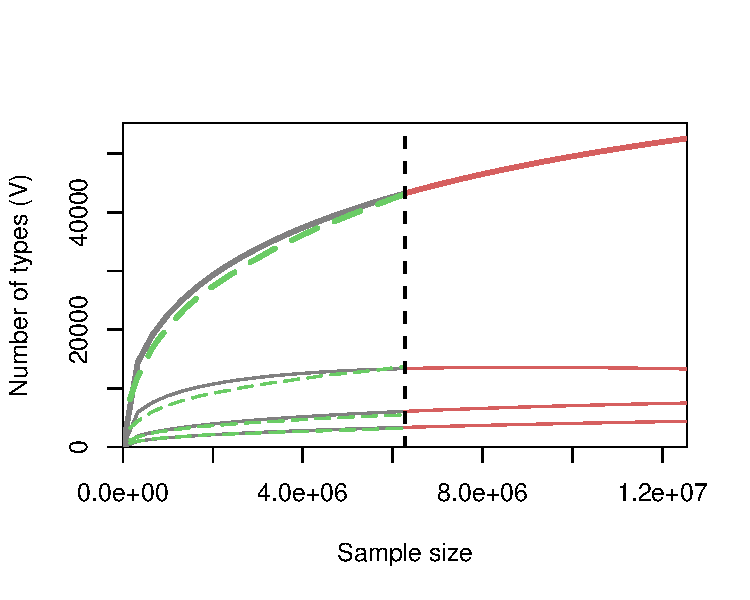
\includegraphics[scale=.6]{figures/df.growth.intrextr-3.5.pdf}
    \caption{Type-token growth curve, including inter- (grey) and extrapolation (red) based on a finite Zipf-Mandelbrot LNRE model \citep[Large Numbers of Rare Events Model][]{evert_simple_2004}. From top to bottom, the lines show the total numbers of types, as well as the numbers of types that occur at most 3, 2, and 1 times, respectively (i.e., tris legomena $V_3$, dis legomena $V_2$, and hapax legomena $V_1$).}
    \label{fig:df.growth.intrextr}
  %\end{minipage}
  \hfill
\end{figure}

\begin{figure}[h]
  \centering
%  \begin{minipage}[t]{0.9\textwidth}
    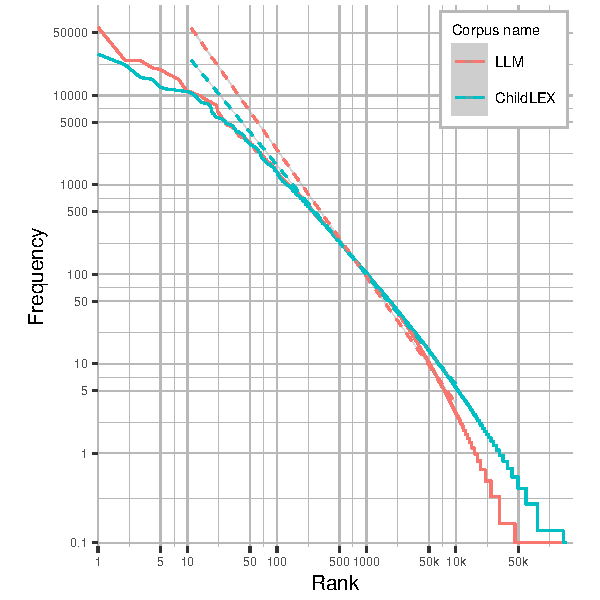
\includegraphics[scale=.8]{figures/rankplot-normal-3.5-2.pdf}
    \caption{Zipf's law plot, showing differing slopes across the LLM and ChildLex corpora. The slopes are fitted to a subset of words with a frequency between 10 and 10,000. }
    \label{fig:rankplot-normal}
  %\end{minipage}
\end{figure}

\begin{figure*}[t]
    \centering
    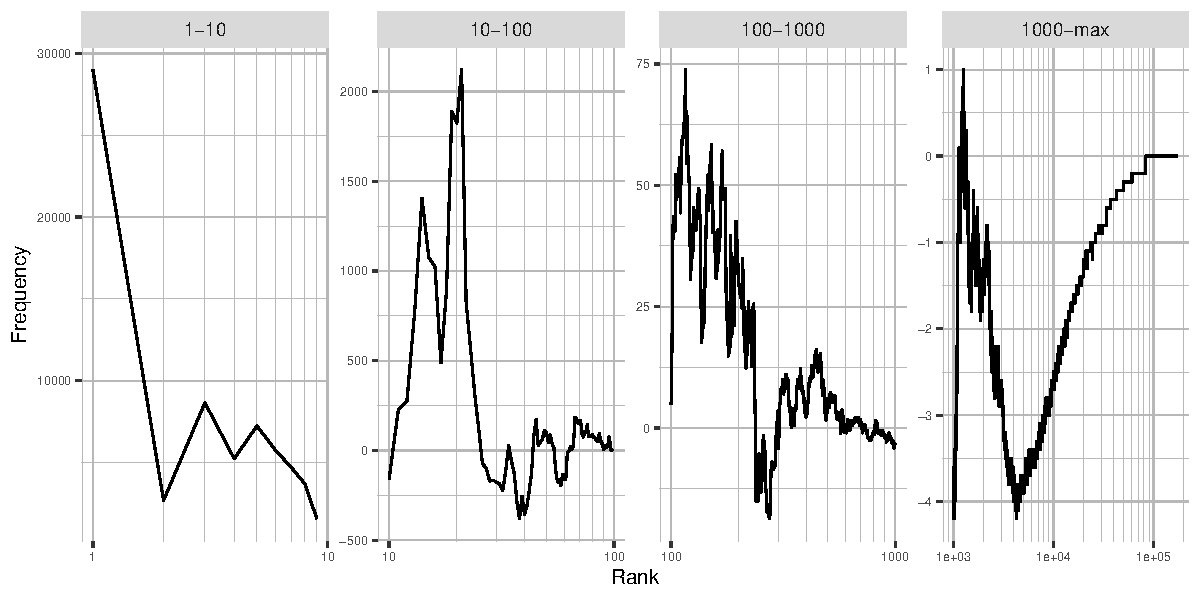
\includegraphics[scale=.8]{figures/rankplot-difs-3.5-2.pdf}
    \caption{Differences between frequencies calculated based on the LLM and ChildLex corpora (i.e., the difference between the curves from Figure \ref{fig:rankplot-normal}).}
    \label{fig:rankplot-difs}
\end{figure*}


\subsection*{Detailed comparison to ChildLex}

Despite apparent differences, such as in lexical richness, we find a relatively high correlation between word frequency measures from ChildLex and the LLM-based corpus (r = 0.88). This correlation stays at .88 when we include all words not in the other corpus and set their frequency to .1 (see Figure \ref{fig:cor1}). The high correlation and the scatter plot illustrate the high similarity of the two measures. However, comparing frequencies in this way also allows us to look at the words that differ in frequency the most in both directions. We find that LLM-specific words sometimes result from spillover effects from the most likely predominant English training data. For example, the word "namens" probably directly spills over from the typical phrase to start a story in English: "There was an X called Y" even though "namens" is not typically used in this context as a translation equivalent in German. This result is similar to the observed losses in lexical and morphological richness in automatic machine translation \citep{vanmassenhove_machine_2021}. On the other hand, the word frequencies that stand out in ChildLex are typically associated with narrative storytelling. This finding is unsurprising, as the LLM corpus comprises only summary-like text.  

\begin{figure}[t]
  %\centering
  \centerline{
  %\begin{minipage}[t]{0.9\textwidth}
    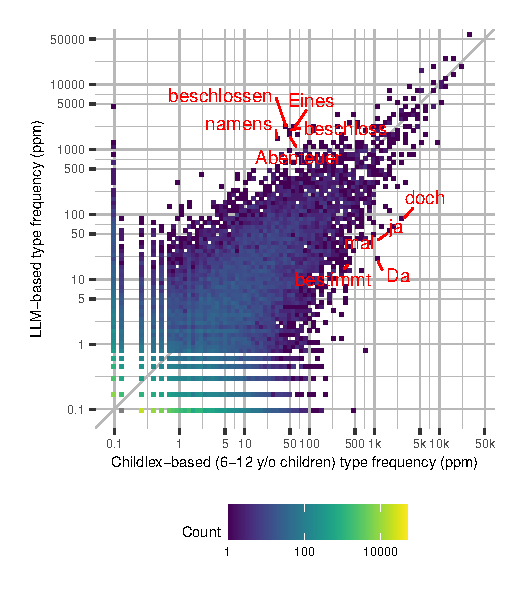
\includegraphics[width=.55\textwidth]{figures/for 6-12ChildLexLLM-3.5-ch-test-3.pdf}}
    \caption{Correlation between LLM-based type frequency (y-axis) and ChildLex-based type frequency (x-axis; dark gray line). The labels show the top five differences on both sides (x-y and y-x). The color gradient of the dots represents the number of data points each dot represents.}
    \label{fig:cor1}
  %\end{minipage}
\end{figure}




\paragraph{Robustness of the word frequency effect against corpus size}

To estimate the robustness of the correlation of the LLM-based and ChildLex frequencies, we re-estimated the LLM-based frequencies based on subsets from the complete corpus, specifically for the words used in the DeveL dataset \citep{schroter_developmental_2017}. For this analysis, we started with the first LLM texts generated based on a prompt using the first book. After that, we successively added the texts from the next book and re-estimated the correlations for each subset (see Figure \ref{fig:partial_data}A). The curve shows a logarithmic increase in the correlation, indicating a substantial increase in the similarity of the two measures within the first 50 texts. After that, the increase in similarity is weaker, ending up at a correlation coefficient of just below .75. We further inspected whether this shape is indeed logarithmic, by taking all the correlation quotients on the y-axis and the numbers of texts from the x-axis, and computing a correlation between them (r = .71) and then computing this correlation again but taking the log of the numbers of texts from the x-axis instead (.94). This second correlation is much higher, indicating that the increase is indeed more logarithmic. Figure \ref{fig:partial_data}B also reports this correlation of .94 in the top left corner. 

\begin{figure*}[ht]
    \centering
    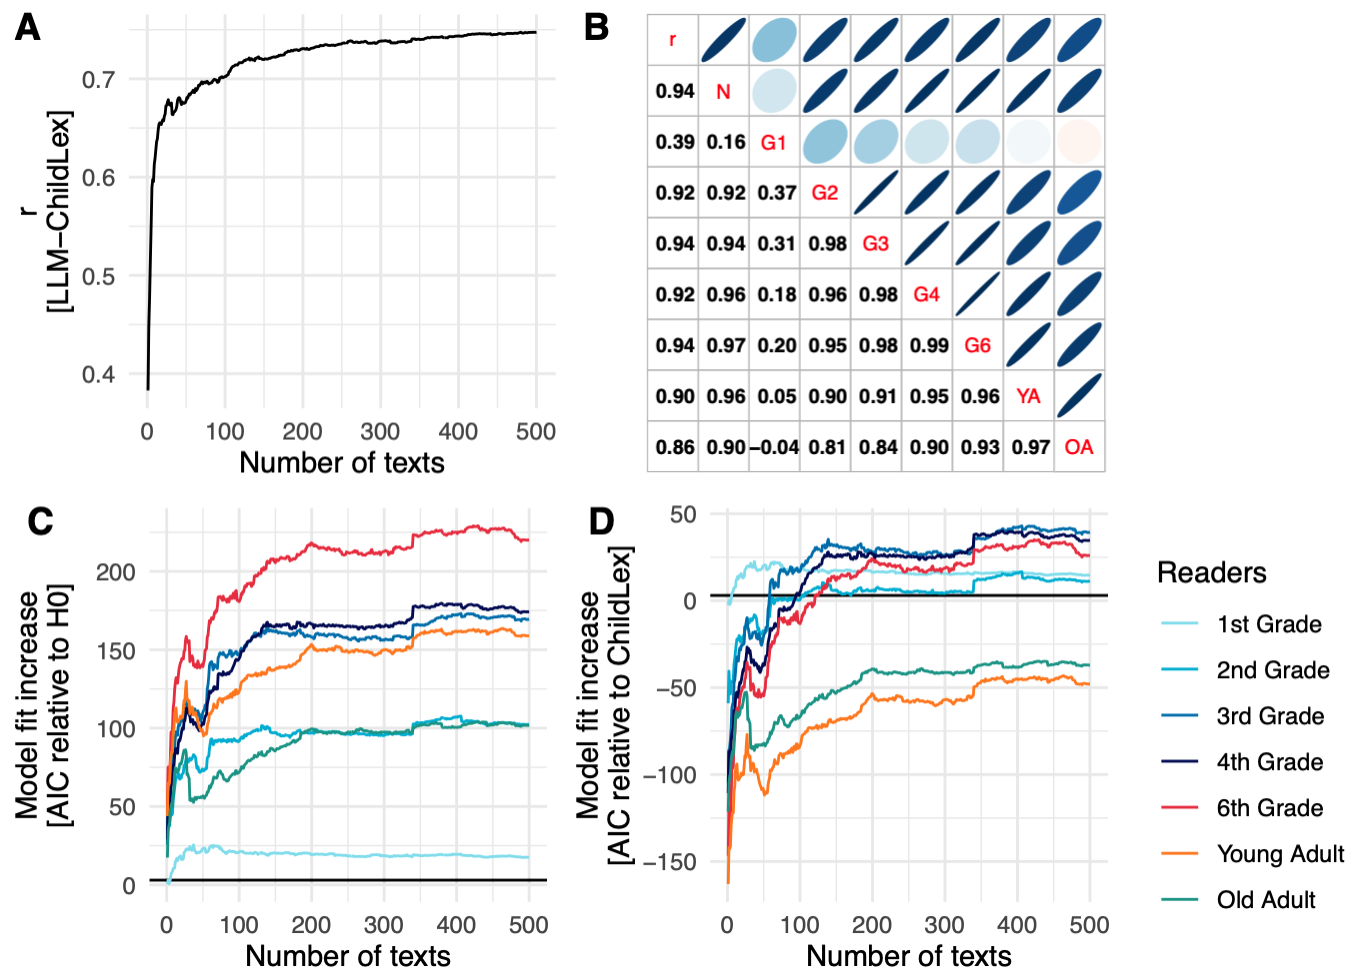
\includegraphics[scale=.28]{figures/partial_fig.png}
    \caption{Partial LLM corpus analysis investigating the correlation between ChildLex corpus and reading performance. (A) Subset-based estimation of the correlation between LLM-based type frequency and ChildLex type frequency (y-axis). We estimated the correlation 500 times based on an LLM-based frequency extracted from a corpus that included only the first book. After that, we included all generated text from one additional book until all books were included. Note that this analysis was implemented for the words used in the DeveL dataset. (B) Pearson correlation matrix investigating the partial data curves from A and C. \textit{r} represents the correlations from A; \textit{N} represents the log-transformed number of stories (i.e., x-axis from A, C, or D); \textit{G1-6}, represent the AIC differences from Grade 1 to 6 shown in C; \textit{YA} and \textit{OA} represent the young and old adults AIC differences shown in C. Lower matrix shows the correlation coefficient r and the upper matrix the color coded (blue: positive correlation; white: no correlation; red: negative correlation) correlation silhouettes (narrow silhouettes indicate high and wide silhouettes indicate low correlations). (C) AIC difference of a Linear Mixed Model (LMM) that included word frequency measures estimated on a subset of the LLM-generated corpus (i.e., same subsets as in A) to the model without a frequency estimate included and (D) when the baseline model included the ChildLex frequency.}
    \label{fig:partial_data}
\end{figure*}


\subsection*{Evaluating LLM-based word frequency estimates based on reading performance}

For the reading performance-based evaluation of the LLM-generated frequency measure, we used three approaches: (i) repeatedly calculating linear models with reaction time as the dependent variable and with word frequencies as the predictor of interest, for incrementally increasing text sizes. We did this in the same way as for the robustness analysis from \ref{fig:partial_data}A) above, starting with texts based on the first book only, and continuing until all texts from all 500 books were added. These models also controlled for other factors that potentially affect reading performance, but that are of no interest for the current study \citep[OLD20, ][]{yarkoni_moving_2008,hawelka_beyond_2013}; age-of-aquisition, \citep{weekes_effects_2006}; letter length \citep{gagl_sources_2015, huestegge_oculomotor_2009, marinus_variability_2010, zoccolotti_word_2005}; uni-, bi- and tri-gram frequency). After calculating the effects from the linear model, we estimated the model fit based on the Akaike Information Criterion \citep[AIC, ][]{akaike_new_1974}. To estimate the AIC, we compared the model to a baseline model without a frequency measure. Higher AIC differences indicate more increase in model fit when we added frequency to the baseline model. (ii) The same partial analysis but in the baseline model, we included the ChildLex-based frequency measure, allowing a comparison that shows the increase in model fit over and above the current state of the art. (iii) Comparing LLM frequency measures based on the complete corpus to multiple, alternative frequency measures, including ChildLex (similar as in ii) and two adult corpora, a book-based corpus \citep[DWDS][]{heister_dlexdb_2011}, and a Subtitle-based corpus \citep[SUBTLEX][]{brysbaert_word_2011}. For both evaluations, we used an existing dataset that includes lexical decision performance measures, in our case, response times, from children in first, second, third, fourth, and sixth grade. This dataset also includes a sample of young and older adults \citep[DeveL, for more details, see ][]{schroter_developmental_2017}. The latter two samples allow us to investigate the specificity of the corpus for child readers. Here, we expect that the frequency measures from adult corpora (DWDS and SUBTLEX) should be more precise in describing adult data, and vice versa, the child-directed frequency measures should describe the data of the beginning readers better (ChildLex and the LLM-based frequency). 

\paragraph{Model fit estimations based on partial sample corpus frequency measures}

Here, we evaluated to what extent frequency measures based on corpus subsets result in a lower model fit. Thus, we increased the corpus size (same as above), estimated the frequency, and measured the model fit change when introducing the established frequency measures compared to a model without the measure. We implemented this, starting with the texts from the first book. Ultimately, we can compare the absolute AIC difference values (i.e., AIC from the model with the new frequency predictor minus the AIC based on the model without the predictor; the higher, the better the model fit) from all estimated frequencies and all reading groups (1st-4th Grade, 6th Grade, young and old adults; N tests = 500; see Figure \ref{fig:partial_data}C). We rely on model comparison methods using linear regression models and the AIC, a measure optimal to investigate model fit change for newly introduced parameters. Note that a change in three AIC points is a significant model fit increase (i.e., the black horizontal line in Figure \ref{fig:partial_data}C and D; all AICs above show a significant increase in model fit).

The clear finding of this partial corpus analysis is that the reading performance can be explained better based on frequency measures that we estimated from larger corpora (Figure \ref{fig:partial_data}C). We find an increase in the AIC difference in all age groups, although the trend is much smaller in the youngest readers from Grade 1 (compare correlations of the size of the corpus - N - and Grade 1 - G1 - in contrast to the more older readers in Figure \ref{fig:partial_data}B). Nonetheless, all analyses, except for the frequency measures based on very small corpora (Number of books < 5) predicting the reaction times of Grade 1 readers, showed a significant increase in model fit. Correlations of AIC differences with increasing corpus size of all our groups of readers also showed that in Grade 1, the pattern differed from all other groups (Figure \ref{fig:partial_data}B). In addition, groups with similar age (e.g., Grade 2 vs. Grade 3) had higher correlations (r range from .96 to .99) compared to comparisons with substantial age differences (e.g., Grade 2 vs. old adults; r = .81). Finally, the partial analysis that estimated the AIC differences against a baseline model including the ChildLex frequency as a predictor, showed that only linear models that predicted the reaction times of young readers (Grade 1-6) had an additional model fit increase based on the inclusion of the LLM-based frequency (see Figure \ref{fig:partial_data}D). Models describing adult data did not benefit from introducing the LLM-based frequency measure. Also, we observed that for young readers, larger corpus sizes are needed for the frequency estimation to produce a frequency estimate with higher descriptive power (Grade 1: 6 books; 2: 103; 3: 59; 4: 95; 6: 121; see Figure \ref{fig:partial_data}D).

\begin{figure}[ht]
    \centering
    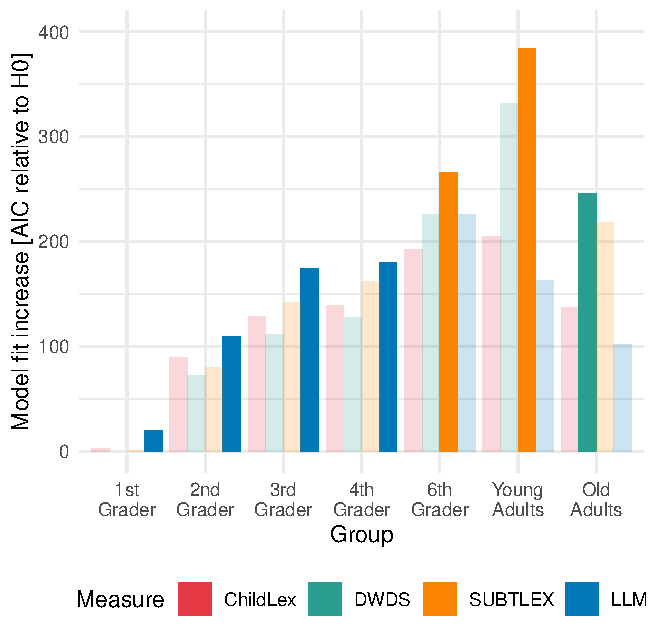
\includegraphics[scale=.7]{figures/lexica-comp.pdf}
    \caption{Evaluation of the LLM-based frequency measure based on reading performance (lexical decision times) of beginning readers (Grades 1, 2, 3, 4, and 6), young and old adults. AIC difference based on analysis using the entire LLM-based corpus for the frequency estimation, ChildLex-based frequency, DWDS-based frequency, and the SUBTLEX-based frequency measure for all age groups. We only highlighted the model with the highest model fit (i.e., the largest AIC difference).}
\label{fig:modelcomprt}
\end{figure}

\paragraph{Comparing model fit estimations from LLM-based to classical frequency measures}

As described above, we compared the new LLM-based frequency to other frequency measures previously used to describe the word frequency effect in visual word recognition performance. Here, we found that the AIC difference is largest for the LLM-based frequency for young readers (Grade 1-4; see Figure \ref{fig:modelcomprt} lower panel), indicating that the LLM-based frequency measure describes the frequency effect best. For the Grade 6 and young adult readers, we found that the SUBTLEX frequency measure, which relied on subtitles from films and TV shows, had the highest model fit increase. Finally, the book and newspaper-based frequency measures from the DWDS corpus only showed the highest model fit in older adults (see Figure \ref{fig:modelcomprt} lower panel). 

\section*{Discussion}

This article showed that, when estimating word frequency, text corpora from Large Language Models (LLM) can be helpful for psycholinguistic research. We generated a corpus based on multiple LLM prompts. In each prompt, we asked the model to summarize a book written for children in a child-specific language. Critical for the evaluation was that we used the book titles from an established German corpus based on children's books \citep[ChildLex; ][]{schroeder_childlex_2015}, so we had the opportunity to directly compare the frequency measures from the original ChildLex corpus and the LLM-based corpus. There were three main findings: (i) The LLM corpus had fewer types (i.e., less distinct words), and relatively frequent words comprised a more significant part of the LLM-based corpus. (ii) LLM-based frequencies correlated strongly with ChildLex frequencies, showing a substantial similarity of the measures, although both corpora had a substantial number of words specific for one corpus. (iii) In a reading-performance-based evaluation, we found that the LLM-based frequency describes the performance of younger readers better than word frequency estimates based on published children's books. Thus, the present exploration indicates that one can use LLMs to create meaningful corpora to measure word frequency despite the substantial differences in word types included in the corpora.  

\subsection*{Low richness of LLM corpus}
The central characteristic of our LLM-based corpus, compared to ChildLex, is that it includes fewer types, and frequent types occur very often. This finding could result from the limitations of current LLMs or our prompt design. Word count currently limits the text generated by the model. Thus, LLM-based texts are much shorter than the original books. We prompted the LLM multiple times to compose a text based on each book's title, which allowed us to generate a substantial number of words concerned with the topic from each ChildLex book. The result that the LLM corpus had a relatively high number of high-frequency types (i.e., the LLM uses fewer words, but these words are used repeatedly) could result from our prompting strategy. Such that LLMs generate words central to a book (e.g., \textit{wand} in Harry Potter) more often, resulting from our repeated prompting. However, overall, the usage of function words is lower, as well as words types such as "sagt", which are indicative of direct speech. Another reason for the low number of unique types could be the result of our child-directed prompt design (i.e., we added "for children" to the prompts). Here, the interpretation would be that the representations of the model could directly reflect a relatively simple type of child-directed language. Of course, other text types besides books are present in the training data. In contrast, books represent adult language directed to children, i.e., potentially following a learning agenda \citep[e.g., ][]{cain_matthew_2011}. Here, authors could increase the vocabulary used in the books to establish the usage of words common to adults but not known to all young readers yet (i.e., an adult vocabulary bias). Also, because vocabulary increases with literacy onset \citep{cunningham_vocabulary_2005}, LLM-generated text might better represent young readers' vocabulary. However, using LLM-text in education could also even benefit vocabulary growth with enough careful consideration \citep[see ][ for a LLM text specific opportunities]{kasneci_chatgpt_2023}. 

In the future, we can expect longer texts from newer LLM versions, as one primary objective in LLM development is increased text length. So, multiple prompts might no longer be necessary. Another way to increase the number of types could be to vary the model's temperature (i.e., that increases or decreases the "creativity" of the model output) or to orchestrate a set of prompts to evoke different narrative text styles, such as "write a story about", or "write an introduction to a novel / write the first chapter…". In this first analysis, we did not attempt to optimize our prompt design to generate a more narrative style with plausible narrative elements and structures. Our main objective was to distinguish generated text for constructing psycholinguistic resources and not to optimize text quality characteristics. To understand the general differences between AI-generated stories and children's stories, one must look at textual characteristics not picked up by lexical or grammatical statistics, entropy, complexity, and others. Some future directions could include computing semantic similarity scores based on word embeddings, e.g., BERT, training understandable models to discriminate texts, and focusing on elements, such as rhetorical devices (https://huggingface.co/browndw/docusco-bert). Nevertheless, despite this difference in the types produced by the LLM, the correlation between word frequency estimates from the LLM and book-based corpora indicates a high overall similarity of the corpora on the word level.

\subsection*{Correlations between LLM- and book-based word frequencies}

The correlation between the word frequency estimates of the book- and LLM-based corpus is substantial and robust to the size of the corpus used for the estimation. For the DeveL-selection of about 1000 words, after an initial exponential correlation increase within the first 20\% of the corpus (i.e., r increased from around .4 to around .7), only an incremental increase was observed after that (i.e., r increased from around .7 to around .75). These findings indicate high similarity in the frequency estimates for the words included in both corpora. The main advantage of a larger corpus is that the number of words for which one can estimate word frequency is higher. So, the coverage of larger corpora would be better, but the similarity increase to a classical book-based corpus would only be incremental. 

\subsection*{Reading performance-based evaluation of LLM- and book-based word frequencies}

For the evaluation based on reading performance, we used the lexical decision data of the DeveL (i.e., response times of young readers from Grades 1-6, young and older adults). In the first analysis, we found that the model fit, in describing the response time data, increased when including a word frequency estimate based on only a fraction of the full LLM-corpus (N $<$ 10 texts) for all age groups. Nonetheless, increasing the corpus size also increased the model fit further. For all but Grade 1 readers, the increase in model fit with a larger corpus was highly similar to the increase in the correlation between LLM- and book-based corpora described above (r range: .86 - .94). The difference for Grade 1 was that model fit analysis peaked after about 10\% of the corpus, with an incremental decrease of model fit for word frequencies based on larger corpora (i.e., when N $>$ 100). Similarly, we compared the model fit increase for LLM-based frequencies based on partial corpora to a model that already included the ChildLex book-based word frequency estimates. Here, we investigated whether the new LLM-based frequency explains variance over and above the classical frequency estimates. Most notably, this was the case for the Grade 1 readers after only a fraction of the texts included (N $<$ 10). For Grades 2-6 readers, an increased model fit was found when the LLM-corpus size was much larger (Grade 2: N $>$ 100; Grade 3: N $>$ 50; Grade 4: N $>$ 100; Grade 6: N $>$ 120). No additional variance was explained, when the ChildLex frequency was already included, for the two adult groups. In a third analysis, we used the frequency estimate based on the entire LLM corpus and compared the model fit for each age group separately, again with ChildLex, but also to two frequency measures based on adult corpora: DWDS \citep{heister_dlexdb_2011} and SUBTLEX \citep{brysbaert_word_2011}. Each model included only one frequency measure, so we used four analyses for each group, which allowed us to investigate which measure explains most of the variance in lexical decision response times. We found for Grades 1-4 that our LLM-based frequency had the highest fit. For Grade 6 and young adults, the SUBTLEX frequency, based on film subtitles, had the highest fit. For old adults, the book-based DWDS corpus had the highest fit.   

This pattern of results offers three critical insights: (i) For young readers, the LLM-based word frequency best describes reading performance and variance over and above the classical book-based frequencies. This finding could indicate that the word frequency effect that describes the process of accessing the mental lexicon \citep{brysbaert_word_2018, brysbaert_word_2011, gregorova_access_2023} is better described based on a corpus that has fewer types that are more frequent. (ii) The highly expected smaller lexicons in Grade 1 readers \citep[e.g.][]{segbers_how_2017} are reflected in the better fit of LLM word frequency estimates when the corpus is small. This observation suggests that investigating the word frequency effect at the beginning of literacy acquisition demands an estimation of word frequency based on smaller corpora with child-specific content, in our case, generated by an LLM. (iii) For older readers of Grade 6 and young adults, the subtitles-based measure was best, and the adult book- and newspaper-based corpus for the older adults. This finding indicates that the child-specific prompts that generated the LLM corpus resulted in a corpus that best describes children's data. In contrast, the adult corpora were better for the older readers, suggesting child specificity of the LMM corpus.  

Overall, these results suggest that the LLM-based frequency estimates better represent the lexicon of young readers compared to children's books. This also suggests that LLMs could potentially provide a new paradigm for generating corpora representing other age and language groups, potentially generating resources that are currently unavailable but desperately needed \citep[e.g., frequency measures in underrepresented languages][]{gagl_eye_2022, blasi_over-reliance_2022}. 

\subsection*{Limitations and future research}

The lexical richness and word reading times are simplistic qualities of text compared to the cultural, social, and ethical themes and pedagogical considerations underlying children's books. This study does not discuss the higher-level semantics or syntax of the books analyzed here. Also, the study does not investigate whether LLM texts can be used to assess these qualities. However, the generated texts are available (find here: ADD URL) and can be used for such investigations. In general, our study shows potential for language development research. Specifically, explained variation in word reading times depends much on the way in which lexical properties are quantified, including word frequencies. We showed that LLM text contains atypical patterns, such as the spillover effects from English to German or numerous words found only in the LLM-based corpus but not in the book corpus. This insight should be taken seriously, especially when LLMs play a role in wider societal and digital discourses. For example, we highly recommend more in-depth, higher-level analysis before using generated texts in settings involving vulnerable participants (e.g., in the context of school or the wider public). 

Other important factors include e.g. authorship and text types. ChildLex, for example, is composed of texts written solely by adults (albeit for children), and thus cannot directly represent either child-directed speech in regular discourse (i.e., parent-child or teacher-child interaction) nor child-produced speech. Also, specific text characteristics, including the production of summaries (LLM) vs. narrations (ChildLex) are important. Furthermore, it seems likely that text generated in a specific language or a specific register, for which little training data is available, might have lower quality than cases for which more training data is available. 

\section*{Conclusions}

Surprisingly, the generation of texts specifically directed to children from LLMs allows us to estimate word frequency that is similar to existing resources, but more importantly, the newly generated frequencies represent the lexicon of young readers better than any resource before. This striking finding opens up numerous new possibilities for investigating the word frequency effect, i.e., one of the most important effects in psycholinguistics research \citep{brysbaert_word_2018} and beyond \citep{gregorova_access_2023}. Still, caution is important when trying to understand the possibilities of LLMs for language development research. LLMs deviate in important ways from natural language acquisition pathways. The unnaturalness of LLMs results, on the one hand, in some very surprising patterns of language use (c.f. \citep{vanmassenhove_machine_2021}, but on the other hand, in language that is remarkably like natural language, and therefore useful to study certain specific processes such as, for example, patterns of word processing cost. The patterns we exposed here may change soon (i.e., with new versions of LLMs). Nonetheless, it will be important to be able to quantify and compare the ways in which specific elements of text and reading correlate.  

\section*{Declarations}

\textbf{Funding} This research was supported by the University of Cologne. 

\textbf{Conflicts of interest/Competing interests} We have no conflicts of interest to disclose. 

\textbf{Ethics approval} Not applicable. 

\textbf{Consent to participate} Not applicable. 

\textbf{Consent for publication} Not applicable. 

\textbf{Availability of data and materials} Data and materials are available on OSF, see \href{www.osf.com}{here}.

\textbf{Code availability} Code is also available on OSF, see \href{www.osf.com}{here}.

\textbf{Authors' contributions} 

Conceptualization
All authors previously worked on related issues in different research domains. This helped to clarify issues and build ideas to arrive at our design together. 

Data curation
Job Schepens developed an initial system for automatic corpus generation. Benjamin Gagl reimplemented and improved the system. 

Corpus construction and comparison infrastructure 
Job Schepens developed the text analysis, combining corpora, and visualization. 

Evaluation based on reading performance
Job Schepens developed an initial script. Benjamin Gagl implemented the scripts used for statistical modeling and visualization. 

Writing 
A first draft was created by Job Schepens and Benjamin Gagl, with extensive feedback from Nicole Marx. 

Leadership 
Job Schepens and Benjamin Gagl led the project. Nicole Marx provided general guidance. 


%\printbibliography
\newpage
\bibliographystyle{apacite} 
\bibliography{gpt.bib}
\newpage

\appendix

\section{Additional comparisons to ChildLex and Litkey}

Table \ref{words-least} shows the top words from the one corpus that appear the least often in the other corpus. 


% latex table generated in R 4.3.0 by xtable 1.8-4 package
% Thu Oct  5 12:26:56 2023
\begin{table*}[]
\caption{The top frequent words that occur the least often in the other corpus, for all word lengths, and for words with more than 10 characters.}
\centering
\begin{tabular}{rllll}
  \hline
 & ChildLex & ChildLex $>$10 & LLM & LLM $>$10 \\ 
  \hline
1 & Ganz & Wahrscheinlich & Jack & Sattelschlepper \\ 
  2 & Wieso & widersprach & Charaktere & Mäusepension \\ 
  3 & Wahrscheinlich & blitzschnell & Brownie & Schulgespenst \\ 
  4 & Bestimmt & Snorkfräulein & Brumm & aufgewecktes \\ 
  5 & Soll & verächtlich & Poppins & unvergessliches \\ 
  6 & verzog & irgendeinem & Zaubermaus & akzeptierten \\ 
  7 & kreischte & anschließend & Sattelschlepper & Korallenschatz \\ 
  8 & quer & irgendjemand & Fips & Abschlussfeier \\ 
  9 & presste & Zaubereiministerium & Hoppel & verantwortungsvoll \\ 
  10 & Meinst & Entschuldige & Mäusepension & unzertrennliche \\ 
   \hline
\end{tabular}
\label{words-least}
\end{table*}

We repeated the analysis from Figure \ref{fig:cor1} using a corpus containing texts written by children themselves (instead of text written for children). This corpus is much smaller, but the resulting figure, see Appendix Figure \ref{fig:cor2}, shows the same pattern and the most differing words can be explained similarly as well. 

\begin{figure}[h]
  %\centering
  \centerline{
  %\begin{minipage}[t]{0.9\textwidth}
    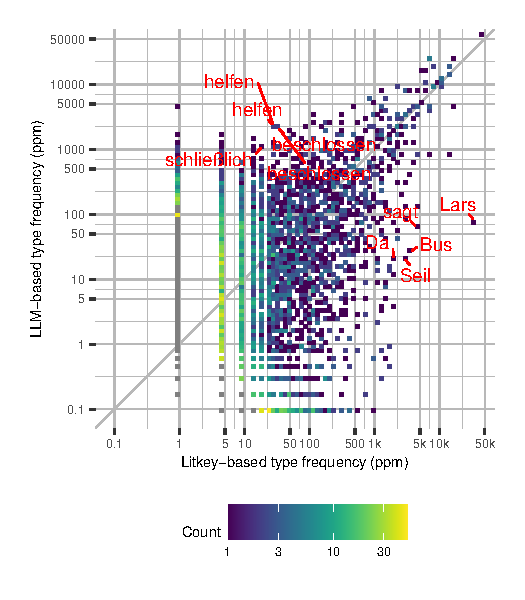
\includegraphics[width=.55\textwidth]{figures/litkeyLLM-3.5-test-3.pdf}}
    \caption{The same as the previous Figure, but showing Litkey-based type frequencies (x axis). The pattern is similar, despite much less available data. }
    \label{fig:cor2}
  %\end{minipage}
\end{figure}

\end{document}